% Options for packages loaded elsewhere
\PassOptionsToPackage{unicode}{hyperref}
\PassOptionsToPackage{hyphens}{url}
\documentclass[
  ignorenonframetext,
]{beamer}
\newif\ifbibliography
\usepackage{pgfpages}
\setbeamertemplate{caption}[numbered]
\setbeamertemplate{caption label separator}{: }
\setbeamercolor{caption name}{fg=normal text.fg}
\beamertemplatenavigationsymbolsempty
% remove section numbering
\setbeamertemplate{part page}{
  \centering
  \begin{beamercolorbox}[sep=16pt,center]{part title}
    \usebeamerfont{part title}\insertpart\par
  \end{beamercolorbox}
}
\setbeamertemplate{section page}{
  \centering
  \begin{beamercolorbox}[sep=12pt,center]{section title}
    \usebeamerfont{section title}\insertsection\par
  \end{beamercolorbox}
}
\setbeamertemplate{subsection page}{
  \centering
  \begin{beamercolorbox}[sep=8pt,center]{subsection title}
    \usebeamerfont{subsection title}\insertsubsection\par
  \end{beamercolorbox}
}
% Prevent slide breaks in the middle of a paragraph
\widowpenalties 1 10000
\raggedbottom
\AtBeginPart{
  \frame{\partpage}
}
\AtBeginSection{
  \ifbibliography
  \else
    \frame{\sectionpage}
  \fi
}
\AtBeginSubsection{
  \frame{\subsectionpage}
}
\usepackage{iftex}
\ifPDFTeX
  \usepackage[T1]{fontenc}
  \usepackage[utf8]{inputenc}
  \usepackage{textcomp} % provide euro and other symbols
\else % if luatex or xetex
  \usepackage{unicode-math} % this also loads fontspec
  \defaultfontfeatures{Scale=MatchLowercase}
  \defaultfontfeatures[\rmfamily]{Ligatures=TeX,Scale=1}
\fi
\usepackage{lmodern}
\ifPDFTeX\else
  % xetex/luatex font selection
\fi
% Use upquote if available, for straight quotes in verbatim environments
\IfFileExists{upquote.sty}{\usepackage{upquote}}{}
\IfFileExists{microtype.sty}{% use microtype if available
  \usepackage[]{microtype}
  \UseMicrotypeSet[protrusion]{basicmath} % disable protrusion for tt fonts
}{}
\makeatletter
\@ifundefined{KOMAClassName}{% if non-KOMA class
  \IfFileExists{parskip.sty}{%
    \usepackage{parskip}
  }{% else
    \setlength{\parindent}{0pt}
    \setlength{\parskip}{6pt plus 2pt minus 1pt}}
}{% if KOMA class
  \KOMAoptions{parskip=half}}
\makeatother
\usepackage{longtable,booktabs,array}
\newcounter{none} % for unnumbered tables
\usepackage{calc} % for calculating minipage widths
\usepackage{caption}
% Make caption package work with longtable
\makeatletter
\def\fnum@table{\tablename~\thetable}
\makeatother
\usepackage{graphicx}
\makeatletter
\newsavebox\pandoc@box
\newcommand*\pandocbounded[1]{% scales image to fit in text height/width
  \sbox\pandoc@box{#1}%
  \Gscale@div\@tempa{\textheight}{\dimexpr\ht\pandoc@box+\dp\pandoc@box\relax}%
  \Gscale@div\@tempb{\linewidth}{\wd\pandoc@box}%
  \ifdim\@tempb\p@<\@tempa\p@\let\@tempa\@tempb\fi% select the smaller of both
  \ifdim\@tempa\p@<\p@\scalebox{\@tempa}{\usebox\pandoc@box}%
  \else\usebox{\pandoc@box}%
  \fi%
}
% Set default figure placement to htbp
\def\fps@figure{htbp}
\makeatother
\setlength{\emergencystretch}{3em} % prevent overfull lines
\providecommand{\tightlist}{%
  \setlength{\itemsep}{0pt}\setlength{\parskip}{0pt}}
% Auto-generated by infrastructure/rendering/_pdf_latex_helpers.py::extract_math_font_preamble.
% Minimal header passed to Pandoc via -H so Beamer slides pick up the same math font
% as the combined-PDF path. Adjust the manuscript's preamble.md to change the font globally.
\usepackage{unicode-math}
\setmathfont{latinmodern-math.otf}

% Slide layout defaults for warning-clean scientific decks.
\usepackage{etoolbox}
\IfFileExists{xurl.sty}{\usepackage{xurl}}{}
\IfFileExists{seqsplit.sty}{\usepackage{seqsplit}}{\newcommand{\seqsplit}[1]{#1}}
\protected\def\breakseq#1{\seqsplit{#1}}
\protected\def\breaktt#1{\begingroup\ttfamily\seqsplit{#1}\endgroup}
\setlength{\emergencystretch}{6em}
\tolerance=5000
\hbadness=10000
\hfuzz=1pt
\setlength{\tabcolsep}{2pt}
\AtBeginEnvironment{longtable}{\tiny\renewcommand{\arraystretch}{0.86}\setlength{\tabcolsep}{1pt}}
\AtBeginEnvironment{tabular}{\tiny\renewcommand{\arraystretch}{0.86}\setlength{\tabcolsep}{1pt}}

% Natbib and cross-reference fallbacks — slides don't load natbib
% or cleveref, but combined-PDF manuscript prose may emit these
% commands. The fallback renders citations as a bracketed key list
% and cross-references as detokenized labels so slides don't fail on
% undefined control sequences or raw underscores. \providecommand is
% a no-op if packages load later.
\providecommand{\citep}[1]{[#1]}
\providecommand{\citet}[1]{#1}
\providecommand{\citealp}[1]{#1}
\providecommand{\citeauthor}[1]{#1}
\providecommand{\citeyear}[1]{#1}
\providecommand{\cref}[1]{\texttt{\detokenize{#1}}}
\providecommand{\Cref}[1]{\texttt{\detokenize{#1}}}
\usepackage{bookmark}
\IfFileExists{xurl.sty}{\usepackage{xurl}}{} % add URL line breaks if available
\urlstyle{same}
% fallback for those not using the hyperref driver hyperxmp:
\makeatletter
\@ifundefined{xmpquote}{\newcommand{\xmpquote}[1]{#1}}{}
\makeatother
\hypersetup{
  hidelinks,
  pdfcreator={LaTeX via pandoc}}

\author{\texorpdfstring{}{}}
\date{}

\begin{document}

\section{Configuration: Schema-Controlled Lexicon, Slots, and Narrative
Moves}\label{configuration-schema-controlled-lexicon-slots-and-narrative-moves}

\begin{frame}[fragile,allowframebreaks]{Configuration: Schema-Controlled
Lexicon, Slots, and Narrative Moves}
The active composition depth is \texttt{deep}. The lexicon exposes 10
category list(s), and the slot declaration expands to 40 concrete token
choice(s). Section switches are evaluated before composition so disabled
sections cannot silently borrow enabled-section claims.

Configuration owns more than vocabulary. It also owns section titles,
narrative moves, method protocol rows, contribution claims, and audit
rules. That makes the manuscript shape visible in one YAML file while
preserving the rule that source code, not hand-edited output, performs
the composition.

The tables in this section expose the declared surface that controls
rendering. They are useful during review because a title change, slot
expansion, or disabled section appears as a small config diff and a
regenerated artifact diff rather than as scattered prose edits.

The configured-field inventory separates 125 explicit YAML path(s) from
11 loader-defaulted path(s). That distinction matters for forks: a field
that appears in the rendered manuscript may be intentionally authored in
\texttt{config.yaml}, or it may be a documented default inherited from
the template.

\begin{figure}
\centering
\pandocbounded{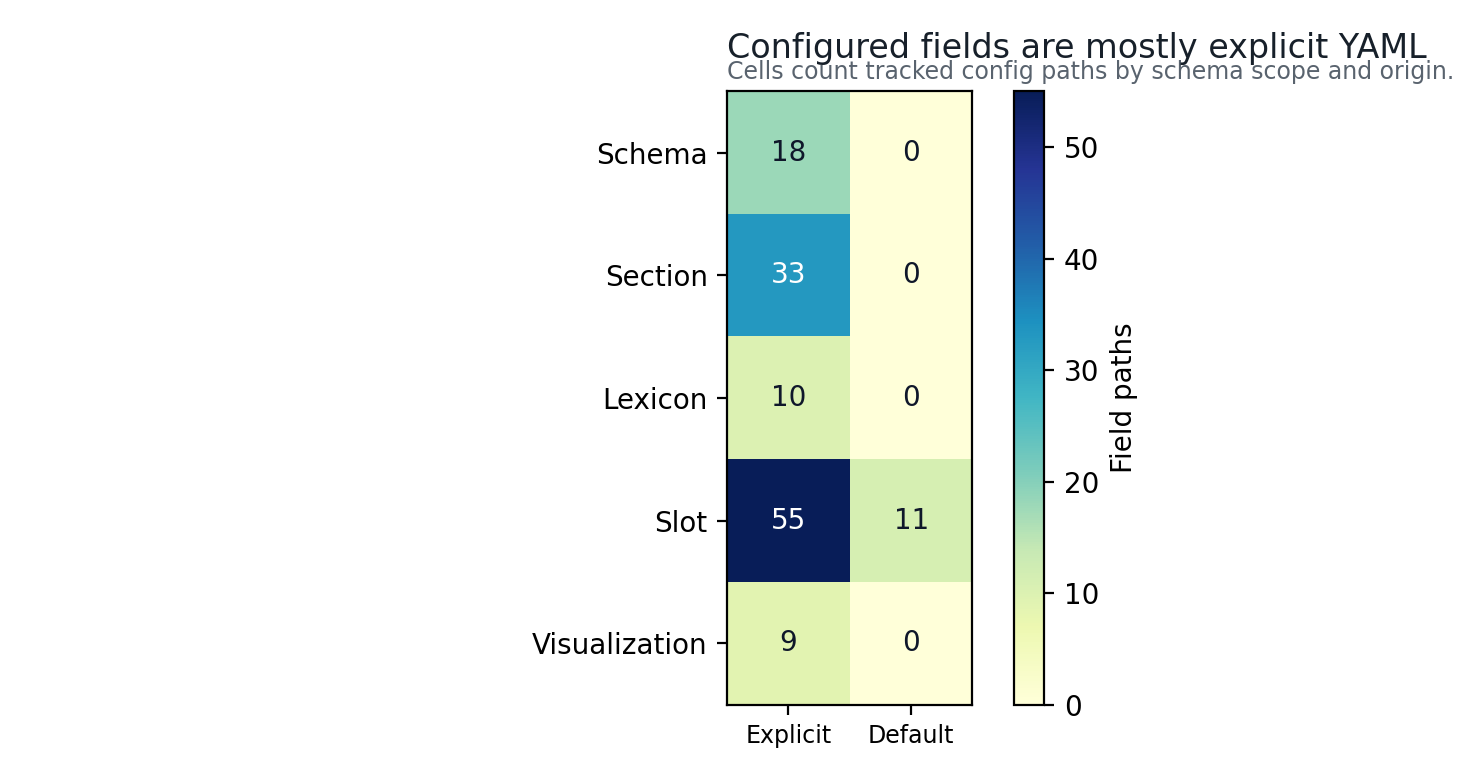
\includegraphics[keepaspectratio,alt={Configured field origin matrix}]{../figures/configured_field_matrix.png}}
\caption{Configured field origin
matrix}\label{fig:configured-field-matrix}
\end{figure}

\begin{figure}
\centering
\pandocbounded{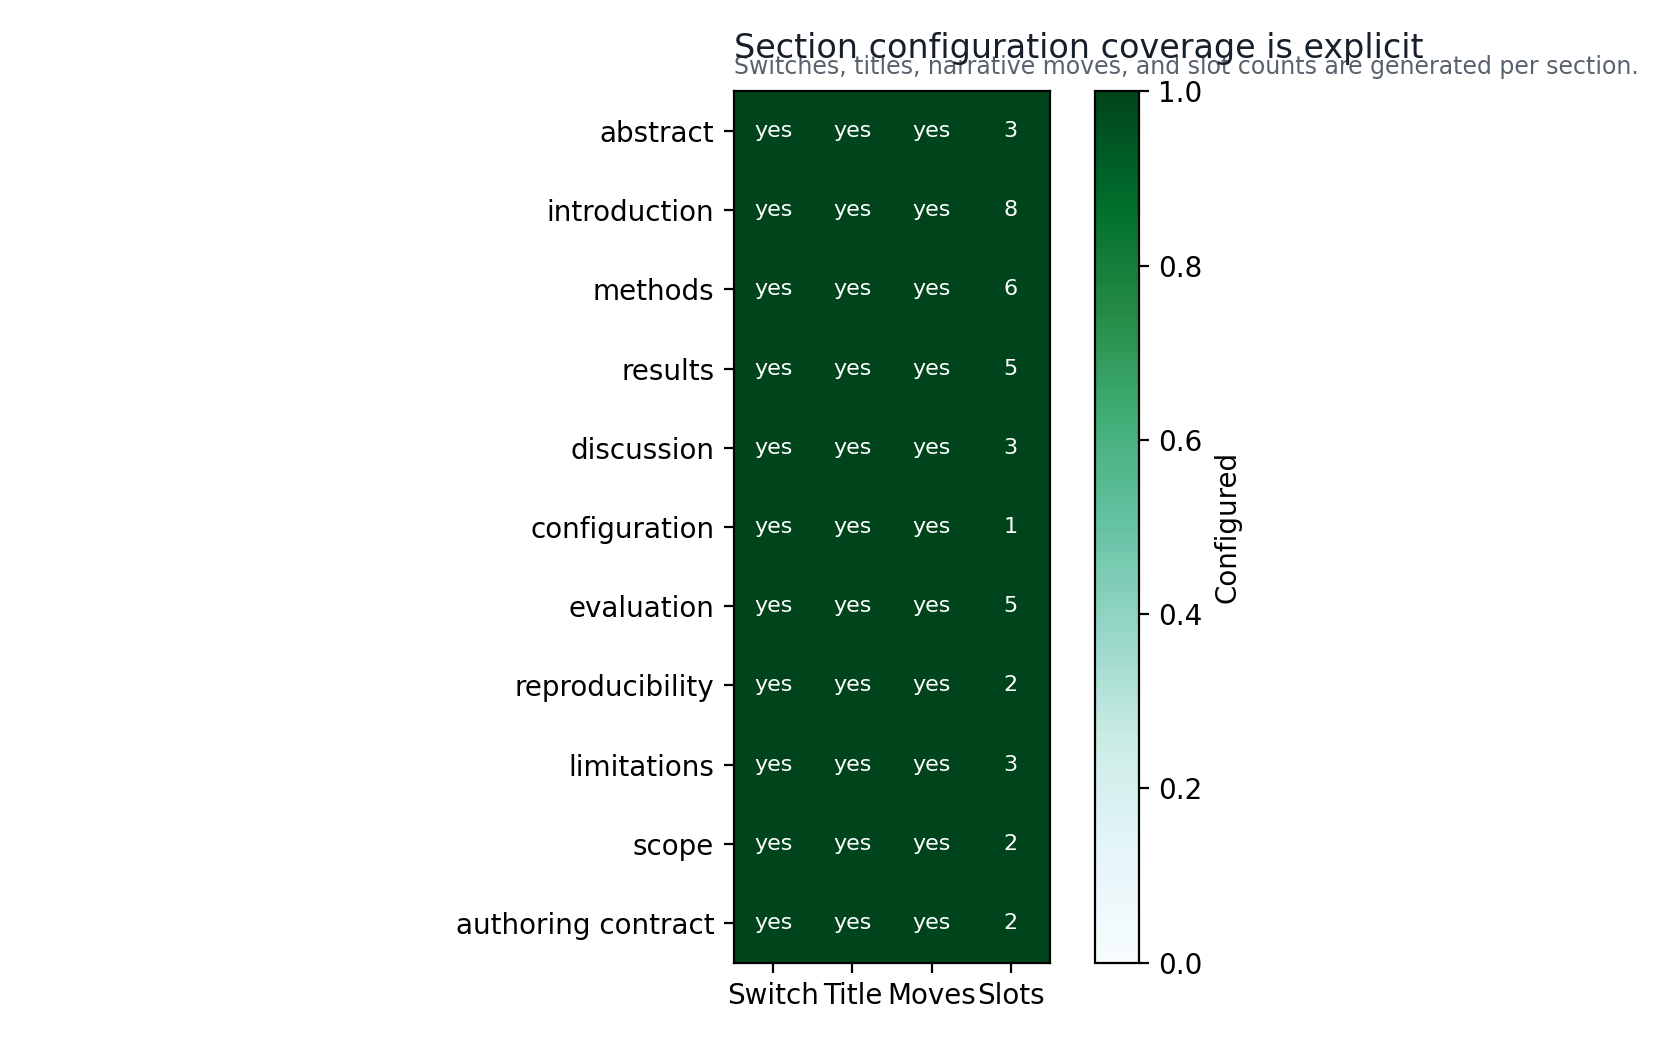
\includegraphics[keepaspectratio,alt={Section configuration heatmap}]{../figures/section_configuration_heatmap.png}}
\caption{Section configuration
heatmap}\label{fig:section-configuration-heatmap}
\end{figure}

\begin{figure}
\centering
\pandocbounded{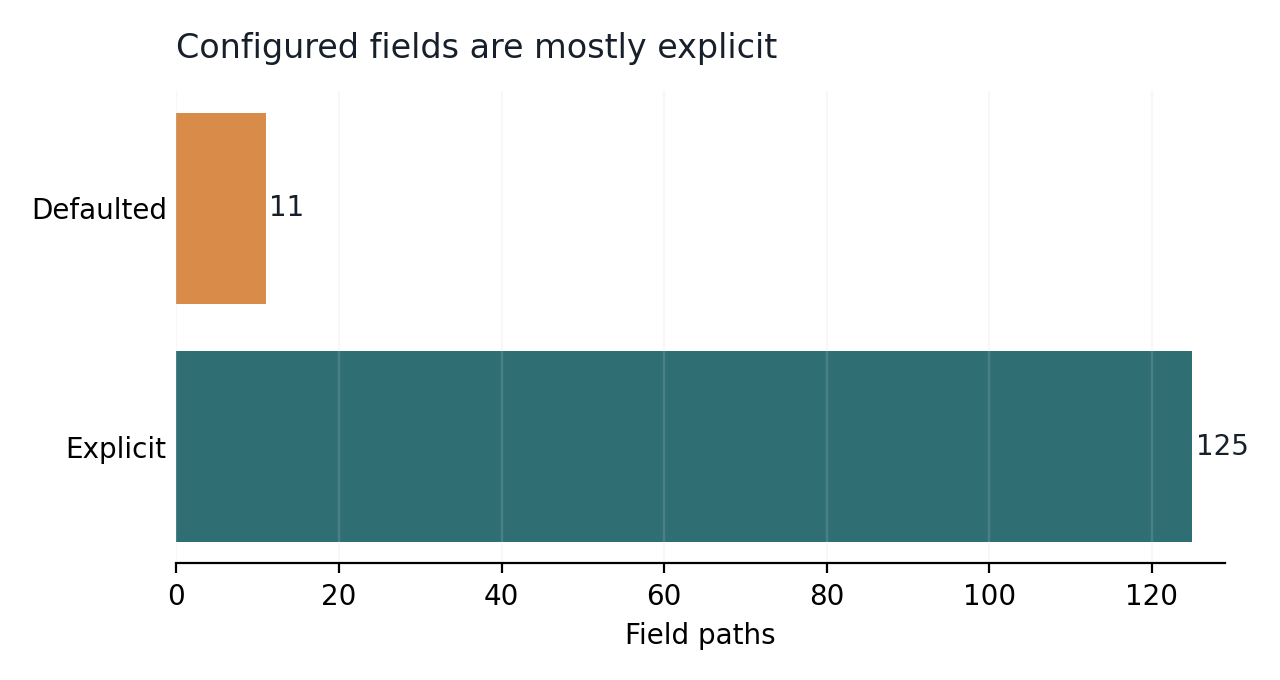
\includegraphics[keepaspectratio,alt={Field origin summary}]{../figures/field_origin_summary.png}}
\caption{Field origin summary}\label{fig:field-origin-summary}
\end{figure}
\end{frame}

\begin{frame}[fragile,allowframebreaks]{Declared Section Titles}
\protect\phantomsection\label{declared-section-titles}
{\def\LTcaptype{none} % do not increment counter
\begin{longtable}[]{@{}
  >{\raggedright\arraybackslash}p{(\linewidth - 4\tabcolsep) * \real{0.3000}}
  >{\raggedright\arraybackslash}p{(\linewidth - 4\tabcolsep) * \real{0.3000}}
  >{\raggedleft\arraybackslash}p{(\linewidth - 4\tabcolsep) * \real{0.4000}}@{}}
\toprule\noalign{}
\begin{minipage}[b]{\linewidth}\raggedright
Section key
\end{minipage} & \begin{minipage}[b]{\linewidth}\raggedright
Rendered title
\end{minipage} & \begin{minipage}[b]{\linewidth}\raggedleft
Enabled
\end{minipage} \\
\midrule\noalign{}
\endhead
\texttt{abstract} & Abstract & True \\
\texttt{introduction} & Introduction: Lexicon as Data and Manuscript as
Build Artifact & True \\
\texttt{methods} & Methods: Source-Owned Token Injection and Conditional
IMRAD Assembly & True \\
\texttt{results} & Results: Provenance, Density, and Resolved Manuscript
Surface & True \\
\texttt{discussion} & Discussion: Accountability Boundaries for
Generated Prose & True \\
\texttt{configuration} & Configuration: Schema-Controlled Lexicon,
Slots, and Narrative Moves & True \\
\texttt{evaluation} & Evaluation: Gate Criteria, QA Probes, and Failure
Discovery & True \\
\texttt{reproducibility} & Reproducibility: Seeded Regeneration and
Artifact Trace & True \\
\texttt{limitations} & Limitations: Non-Claims, Misuse Modes, and Human
Review & True \\
\texttt{scope} & Scope: Related Generators and Responsible Forking &
True \\
\breaktt{authoring\_contract} & Authoring Contract: Human Review and
Forking Obligations & True \\
\bottomrule\noalign{}
\end{longtable}
}
\end{frame}

\begin{frame}[fragile,allowframebreaks]{Configuration Counts}
\protect\phantomsection\label{configuration-counts}
\begin{itemize}
\tightlist
\item
  Seed: \texttt{431}
\item
  Composition depth: \texttt{deep}
\item
  Lexicon categories: \texttt{10}
\item
  Slot rules: \texttt{22}
\item
  Token choices: \texttt{40}
\item
  Enabled sections: \texttt{11}
\item
  Method steps: \texttt{18}
\item
  Design principles: \texttt{13}
\item
  Pipeline phases: \texttt{17}
\item
  Quality probes: \texttt{14}
\item
  Authoring obligations: \texttt{8}
\item
  Explicit configured paths: \texttt{125}
\item
  Defaulted configured paths: \texttt{11}
\item
  Enabled visualization flags: \texttt{7}
\item
  Section-level configured paths: \texttt{33}
\item
  Lexicon-level configured paths: \texttt{10}
\item
  Slot-level configured paths: \texttt{66}
\item
  Narrative moves: \texttt{52}
\item
  Audit rules: \texttt{12}
\item
  Contribution claims: \texttt{9}
\end{itemize}
\end{frame}

\begin{frame}[allowframebreaks]{Configured Field Summary}
\protect\phantomsection\label{configured-field-summary}
{\def\LTcaptype{none} % do not increment counter
\begin{longtable}[]{@{}lr@{}}
\toprule\noalign{}
Measure & Count \\
\midrule\noalign{}
\endhead
Total tracked field paths & 136 \\
Explicit YAML paths & 125 \\
Loader-defaulted paths & 11 \\
Enabled visualization flags & 7 \\
Section-level paths & 33 \\
Lexicon-level paths & 10 \\
Slot-level paths & 66 \\
Visualization-control paths & 9 \\
Top-level schema paths & 18 \\
\bottomrule\noalign{}
\end{longtable}
}
\end{frame}

\begin{frame}[fragile,allowframebreaks]{Configured Field Inventory}
\protect\phantomsection\label{configured-field-inventory}
{\def\LTcaptype{none} % do not increment counter
\begin{longtable}[]{@{}
  >{\raggedright\arraybackslash}p{(\linewidth - 6\tabcolsep) * \real{0.2500}}
  >{\raggedright\arraybackslash}p{(\linewidth - 6\tabcolsep) * \real{0.2500}}
  >{\raggedright\arraybackslash}p{(\linewidth - 6\tabcolsep) * \real{0.2500}}
  >{\raggedright\arraybackslash}p{(\linewidth - 6\tabcolsep) * \real{0.2500}}@{}}
\toprule\noalign{}
\begin{minipage}[b]{\linewidth}\raggedright
Path
\end{minipage} & \begin{minipage}[b]{\linewidth}\raggedright
Origin
\end{minipage} & \begin{minipage}[b]{\linewidth}\raggedright
Scope
\end{minipage} & \begin{minipage}[b]{\linewidth}\raggedright
Summary
\end{minipage} \\
\midrule\noalign{}
\endhead
\texttt{madlib} & explicit & schema & configured field \\
\breaktt{madlib.audit\_rules} & explicit & schema & 12 entries \\
\breaktt{madlib.authoring\_obligations} & explicit & schema & 8
entries \\
\breaktt{madlib.composition\_depth} & explicit & schema & deep \\
\breaktt{madlib.contribution\_claims} & explicit & schema & 9 entries \\
\breaktt{madlib.design\_principles} & explicit & schema & 13 entries \\
\breaktt{madlib.evaluation\_criteria} & explicit & schema & 7 entries \\
\breaktt{madlib.failure\_modes} & explicit & schema & 13 entries \\
\breaktt{madlib.hypothesis} & explicit & schema & Deterministic lexical
injection can generate a complete conditional IMRAD manuscript while
preserving token provenance, section intent, and audit-ready method
evidence. \\
\texttt{madlib.lexicon} & explicit & schema & 10 categories \\
\breaktt{madlib.lexicon.adjectives} & explicit & lexicon & 7 tokens \\
\breaktt{madlib.lexicon.artifacts} & explicit & lexicon & 12 tokens \\
\breaktt{madlib.lexicon.audiences} & explicit & lexicon & 4 tokens \\
\breaktt{madlib.lexicon.constraints} & explicit & lexicon & 5 tokens \\
\breaktt{madlib.lexicon.failures} & explicit & lexicon & 5 tokens \\
\breaktt{madlib.lexicon.measures} & explicit & lexicon & 8 tokens \\
\breaktt{madlib.lexicon.methods} & explicit & lexicon & 5 tokens \\
\breaktt{madlib.lexicon.nouns} & explicit & lexicon & 7 tokens \\
\breaktt{madlib.lexicon.qualities} & explicit & lexicon & 5 tokens \\
\breaktt{madlib.lexicon.verbs} & explicit & lexicon & 7 tokens \\
\breaktt{madlib.method\_protocol} & explicit & schema & 18 entries \\
\breaktt{madlib.narrative\_moves} & explicit & schema & configured
field \\
\breaktt{madlib.narrative\_moves.abstract} & explicit & section & 3
moves \\
\breaktt{madlib.narrative\_moves.authoring\_contract} & explicit &
section & 5 moves \\
\breaktt{madlib.narrative\_moves.configuration} & explicit & section & 3
moves \\
\breaktt{madlib.narrative\_moves.discussion} & explicit & section & 4
moves \\
\breaktt{madlib.narrative\_moves.evaluation} & explicit & section & 4
moves \\
\breaktt{madlib.narrative\_moves.introduction} & explicit & section & 4
moves \\
\breaktt{madlib.narrative\_moves.limitations} & explicit & section & 4
moves \\
\breaktt{madlib.narrative\_moves.methods} & explicit & section & 13
moves \\
\breaktt{madlib.narrative\_moves.reproducibility} & explicit & section &
4 moves \\
\breaktt{madlib.narrative\_moves.results} & explicit & section & 4
moves \\
\breaktt{madlib.narrative\_moves.scope} & explicit & section & 4 moves \\
\breaktt{madlib.pipeline\_phases} & explicit & schema & 17 entries \\
\breaktt{madlib.quality\_probes} & explicit & schema & 14 entries \\
\breaktt{madlib.section\_conditions} & explicit & schema & configured
field \\
\breaktt{madlib.section\_conditions.abstract} & explicit & section &
enabled \\
\breaktt{madlib.section\_conditions.authoring\_contract} & explicit &
section & enabled \\
\breaktt{madlib.section\_conditions.configuration} & explicit & section &
enabled \\
\breaktt{madlib.section\_conditions.discussion} & explicit & section &
enabled \\
\breaktt{madlib.section\_conditions.evaluation} & explicit & section &
enabled \\
\breaktt{madlib.section\_conditions.introduction} & explicit & section &
enabled \\
\breaktt{madlib.section\_conditions.limitations} & explicit & section &
enabled \\
\breaktt{madlib.section\_conditions.methods} & explicit & section &
enabled \\
\breaktt{madlib.section\_conditions.reproducibility} & explicit & section
& enabled \\
\breaktt{madlib.section\_conditions.results} & explicit & section &
enabled \\
\breaktt{madlib.section\_conditions.scope} & explicit & section &
enabled \\
\breaktt{madlib.section\_titles} & explicit & schema & configured
field \\
\breaktt{madlib.section\_titles.abstract} & explicit & section &
Abstract \\
\breaktt{madlib.section\_titles.authoring\_contract} & explicit & section
& Authoring Contract: Human Review and Forking Obligations \\
\breaktt{madlib.section\_titles.configuration} & explicit & section &
Configuration: Schema-Controlled Lexicon, Slots, and Narrative Moves \\
\breaktt{madlib.section\_titles.discussion} & explicit & section &
Discussion: Accountability Boundaries for Generated Prose \\
\breaktt{madlib.section\_titles.evaluation} & explicit & section &
Evaluation: Gate Criteria, QA Probes, and Failure Discovery \\
\breaktt{madlib.section\_titles.introduction} & explicit & section &
Introduction: Lexicon as Data and Manuscript as Build Artifact \\
\breaktt{madlib.section\_titles.limitations} & explicit & section &
Limitations: Non-Claims, Misuse Modes, and Human Review \\
\breaktt{madlib.section\_titles.methods} & explicit & section & Methods:
Source-Owned Token Injection and Conditional IMRAD Assembly \\
\breaktt{madlib.section\_titles.reproducibility} & explicit & section &
Reproducibility: Seeded Regeneration and Artifact Trace \\
\breaktt{madlib.section\_titles.results} & explicit & section & Results:
Provenance, Density, and Resolved Manuscript Surface \\
\breaktt{madlib.section\_titles.scope} & explicit & section & Scope:
Related Generators and Responsible Forking \\
\texttt{madlib.seed} & explicit & schema & 431 \\
\texttt{madlib.slots} & explicit & schema & 22 slot rules, 40 token
choices \\
\breaktt{madlib.slots.authoring\_audience} & explicit & slot & audiences
-\textgreater{} authoring\_contract (1) \\
\breaktt{madlib.slots.authoring\_audience.count} & defaulted & slot &
1 \\
\breaktt{madlib.slots.authoring\_audience.section} & explicit & slot &
authoring\_contract \\
\breaktt{madlib.slots.authoring\_quality} & explicit & slot & qualities
-\textgreater{} authoring\_contract (1) \\
\breaktt{madlib.slots.authoring\_quality.count} & defaulted & slot & 1 \\
\breaktt{madlib.slots.authoring\_quality.section} & explicit & slot &
authoring\_contract \\
\breaktt{madlib.slots.config\_constraint} & explicit & slot & constraints
-\textgreater{} configuration (1) \\
\breaktt{madlib.slots.config\_constraint.count} & defaulted & slot & 1 \\
\breaktt{madlib.slots.config\_constraint.section} & explicit & slot &
configuration \\
\breaktt{madlib.slots.discussion\_adjective} & explicit & slot &
adjectives -\textgreater{} discussion (1) \\
\breaktt{madlib.slots.discussion\_adjective.count} & defaulted & slot &
1 \\
\breaktt{madlib.slots.discussion\_adjective.section} & explicit & slot &
discussion \\
\breaktt{madlib.slots.discussion\_audience} & explicit & slot & audiences
-\textgreater{} discussion (2) \\
\breaktt{madlib.slots.discussion\_audience.count} & explicit & slot &
2 \\
\breaktt{madlib.slots.discussion\_audience.section} & explicit & slot &
discussion \\
\breaktt{madlib.slots.evaluation\_artifact} & explicit & slot & artifacts
-\textgreater{} evaluation (2) \\
\breaktt{madlib.slots.evaluation\_artifact.count} & explicit & slot &
2 \\
\breaktt{madlib.slots.evaluation\_artifact.section} & explicit & slot &
evaluation \\
\breaktt{madlib.slots.evaluation\_measure} & explicit & slot & measures
-\textgreater{} evaluation (3) \\
\breaktt{madlib.slots.evaluation\_measure.count} & explicit & slot & 3 \\
\breaktt{madlib.slots.evaluation\_measure.section} & explicit & slot &
evaluation \\
\breaktt{madlib.slots.intro\_nouns} & explicit & slot & nouns
-\textgreater{} introduction (4) \\
\breaktt{madlib.slots.intro\_nouns.count} & explicit & slot & 4 \\
\breaktt{madlib.slots.intro\_nouns.section} & explicit & slot &
introduction \\
\breaktt{madlib.slots.intro\_verbs} & explicit & slot & verbs
-\textgreater{} introduction (4) \\
\breaktt{madlib.slots.intro\_verbs.count} & explicit & slot & 4 \\
\breaktt{madlib.slots.intro\_verbs.section} & explicit & slot &
introduction \\
\breaktt{madlib.slots.limitation\_failure} & explicit & slot & failures
-\textgreater{} limitations (3) \\
\breaktt{madlib.slots.limitation\_failure.count} & explicit & slot & 3 \\
\breaktt{madlib.slots.limitation\_failure.section} & explicit & slot &
limitations \\
\breaktt{madlib.slots.method\_artifact} & explicit & slot & artifacts
-\textgreater{} methods (2) \\
\breaktt{madlib.slots.method\_artifact.count} & explicit & slot & 2 \\
\breaktt{madlib.slots.method\_artifact.section} & explicit & slot &
methods \\
\breaktt{madlib.slots.method\_constraint} & explicit & slot & constraints
-\textgreater{} methods (1) \\
\breaktt{madlib.slots.method\_constraint.count} & defaulted & slot & 1 \\
\breaktt{madlib.slots.method\_constraint.section} & explicit & slot &
methods \\
\breaktt{madlib.slots.method\_name} & explicit & slot & methods
-\textgreater{} methods (1) \\
\breaktt{madlib.slots.method\_name.count} & defaulted & slot & 1 \\
\breaktt{madlib.slots.method\_name.section} & explicit & slot &
methods \\
\breaktt{madlib.slots.method\_quality} & explicit & slot & qualities
-\textgreater{} methods (2) \\
\breaktt{madlib.slots.method\_quality.count} & explicit & slot & 2 \\
\breaktt{madlib.slots.method\_quality.section} & explicit & slot &
methods \\
\breaktt{madlib.slots.reproducibility\_artifact} & explicit & slot &
artifacts -\textgreater{} reproducibility (2) \\
\breaktt{madlib.slots.reproducibility\_artifact.count} & explicit & slot
& 2 \\
\breaktt{madlib.slots.reproducibility\_artifact.section} & explicit &
slot & reproducibility \\
\breaktt{madlib.slots.result\_artifact} & explicit & slot & artifacts
-\textgreater{} results (2) \\
\breaktt{madlib.slots.result\_artifact.count} & explicit & slot & 2 \\
\breaktt{madlib.slots.result\_artifact.section} & explicit & slot &
results \\
\breaktt{madlib.slots.result\_measure} & explicit & slot & measures
-\textgreater{} results (3) \\
\breaktt{madlib.slots.result\_measure.count} & explicit & slot & 3 \\
\breaktt{madlib.slots.result\_measure.section} & explicit & slot &
results \\
\breaktt{madlib.slots.scope\_audience} & explicit & slot & audiences
-\textgreater{} scope (1) \\
\breaktt{madlib.slots.scope\_audience.count} & defaulted & slot & 1 \\
\breaktt{madlib.slots.scope\_audience.section} & explicit & slot &
scope \\
\breaktt{madlib.slots.scope\_constraint} & explicit & slot & constraints
-\textgreater{} scope (1) \\
\breaktt{madlib.slots.scope\_constraint.count} & defaulted & slot & 1 \\
\breaktt{madlib.slots.scope\_constraint.section} & explicit & slot &
scope \\
\breaktt{madlib.slots.study\_adjective} & explicit & slot & adjectives
-\textgreater{} abstract (1) \\
\breaktt{madlib.slots.study\_adjective.count} & defaulted & slot & 1 \\
\breaktt{madlib.slots.study\_adjective.section} & explicit & slot &
abstract \\
\breaktt{madlib.slots.study\_noun} & explicit & slot & nouns
-\textgreater{} abstract (1) \\
\breaktt{madlib.slots.study\_noun.count} & defaulted & slot & 1 \\
\breaktt{madlib.slots.study\_noun.section} & explicit & slot &
abstract \\
\breaktt{madlib.slots.study\_verb} & explicit & slot & verbs
-\textgreater{} abstract (1) \\
\breaktt{madlib.slots.study\_verb.count} & defaulted & slot & 1 \\
\breaktt{madlib.slots.study\_verb.section} & explicit & slot &
abstract \\
\breaktt{madlib.visualizations} & explicit & visualization & enabled \\
\breaktt{madlib.visualizations.configured\_field\_matrix} & explicit &
visualization & true \\
\breaktt{madlib.visualizations.enabled} & explicit & visualization &
true \\
\breaktt{madlib.visualizations.field\_origin\_summary} & explicit &
visualization & true \\
\breaktt{madlib.visualizations.provenance\_trace\_map} & explicit &
visualization & true \\
\breaktt{madlib.visualizations.quality\_gate\_matrix} & explicit &
visualization & true \\
\breaktt{madlib.visualizations.section\_configuration\_heatmap} &
explicit & visualization & true \\
\breaktt{madlib.visualizations.section\_token\_allocation} & explicit &
visualization & true \\
\breaktt{madlib.visualizations.token\_injection\_flow} & explicit &
visualization & true \\
\bottomrule\noalign{}
\end{longtable}
}
\end{frame}

\end{document}
